\documentclass[titlepage,a4paper]{article}
\usepackage{algorithm}
\usepackage{algpseudocode}
\usepackage{amsmath}

\usepackage{a4wide}
\usepackage[colorlinks=true,linkcolor=black,urlcolor=blue,bookmarksopen=true]{hyperref}
\usepackage{bookmark}
\usepackage{fancyhdr}
\usepackage[spanish]{babel}
\usepackage[utf8]{inputenc}
\usepackage[T1]{fontenc}
\usepackage{graphicx}
\usepackage{float}

\pagestyle{fancy} % Encabezado y pie de página
\fancyhf{}
\fancyhead[L]{Detección de anomalías cardíacas - Demián Fraiman}
\renewcommand{\headrulewidth}{0.4pt}
\fancyfoot[C]{\thepage}
\renewcommand{\footrulewidth}{0.4pt}

\begin{document}
\begin{titlepage} 
    \begin{center}
        \vspace*{3cm} % Ajusta la posición vertical del título
        {\Huge \textbf{Detección de Anomalías Cardíacas}} 
        
        \vspace{2cm}
        {\Large \textbf{Fraiman, Demián}}
        
        \vfill
        {\large 11/02/2025} % Fecha automática
        
        \vspace{2cm}
        
\includegraphics[width=0.3\textwidth]{Logo_de_la_Universidad_de_Buenos_Aires.jpg} % Opcional: agrega un logo institucional
    \end{center}
\end{titlepage}

\tableofcontents % Índice general
\newpage

\section{Introducción}\label{sec:intro}
En la actualidad, las anomalías cardíacas representan la principal causa de muerte en el mundo, por lo que su detección temprana sigue siendo un desafío abierto. Con los avances en redes neuronales y aprendizaje profundo, se ha logrado monitorear pacientes con alta efectividad. Sin embargo, la gran demanda de recursos computacionales y la falta de explicabilidad de estos modelos evidencian la necesidad de diseñar algoritmos más apropiados para esta problemática.

\section{Descripción del Problema}\label{sec:supuestos}

El objetivo de este trabajo es desarrollar un sistema de monitoreo en tiempo real de pacientes mediante un dispositivo electrocardiográfico móvil de una sola derivación. En consecuencia, es necesario diseñar un algoritmo de detección altamente eficiente que permita procesar la señal del usuario de manera continua.  

Además, es importante considerar que no tiene el mismo impacto diagnosticar erróneamente a un paciente enfermo como sano que viceversa, por lo que el algoritmo debe incorporar estrategias que minimicen los riesgos asociados. Asimismo, dada la naturaleza del problema, podemos aprovechar la disponibilidad de los antecedentes médicos y el estilo de vida del usuario para ajustar dinámicamente nuestras predicciones.  

Para abordar esta problemática, utilizaremos una base de datos que contiene información sobre diversos factores relacionados con la salud y las patologías cardíacas. Adicionalmente, trabajaremos con mediciones de señales de ECG, tanto sintéticas como reales, que han sido anotadas y validadas por médicos especialistas.  

A continuación, se presenta la base de datos utilizada:

\begin{figure}[h]
    \centering
    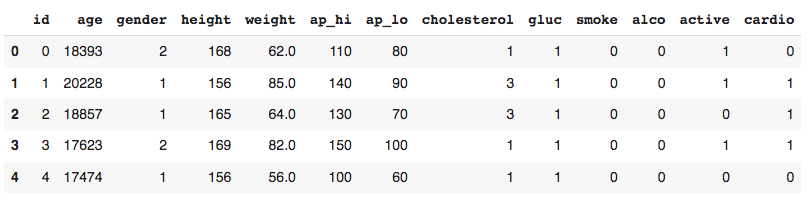
\includegraphics[width=0.8\textwidth]{tabla.png}
    \caption{Tabla de características del usuario utilizadas.}
    \label{fig:mi_figura}
\end{figure}

Las mediciones de ECG fueron tomadas a una frecuencia de muestreo de 140 Hz durante un segundo, por lo que cada registro se almacena en un vector de dimensión 140. Debido a la alta complejidad de la señal y a las limitaciones computacionales del dispositivo, uno de los principales desafíos es encontrar una representación eficiente que permita comprimir la información sin perder consistencia.  


\begin{figure}[h] % [h] indica que se intenta colocar la imagen aquí
    \centering
    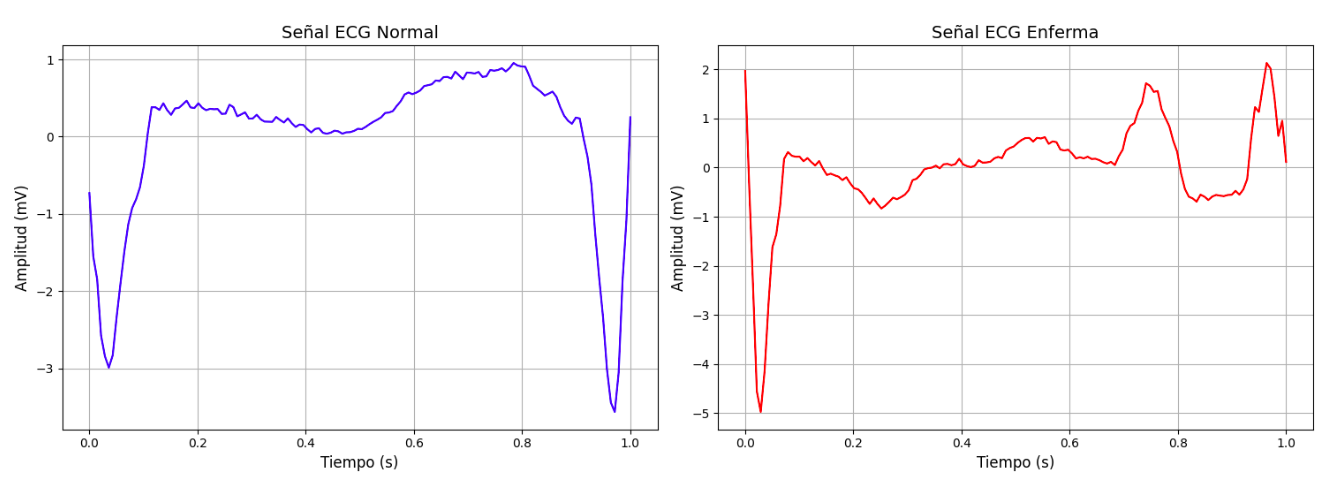
\includegraphics[width=0.9\textwidth]{muestras_reales.png} % Cambia el nombre del archivo
    \caption{Muestras reales de un segundo de señal}
    \label{fig:mi_figura} % Etiqueta para referenciar la figura en el documento
\end{figure}

\begin{figure}[h] % [h] indica que se intenta colocar la imagen aquí
    \centering
    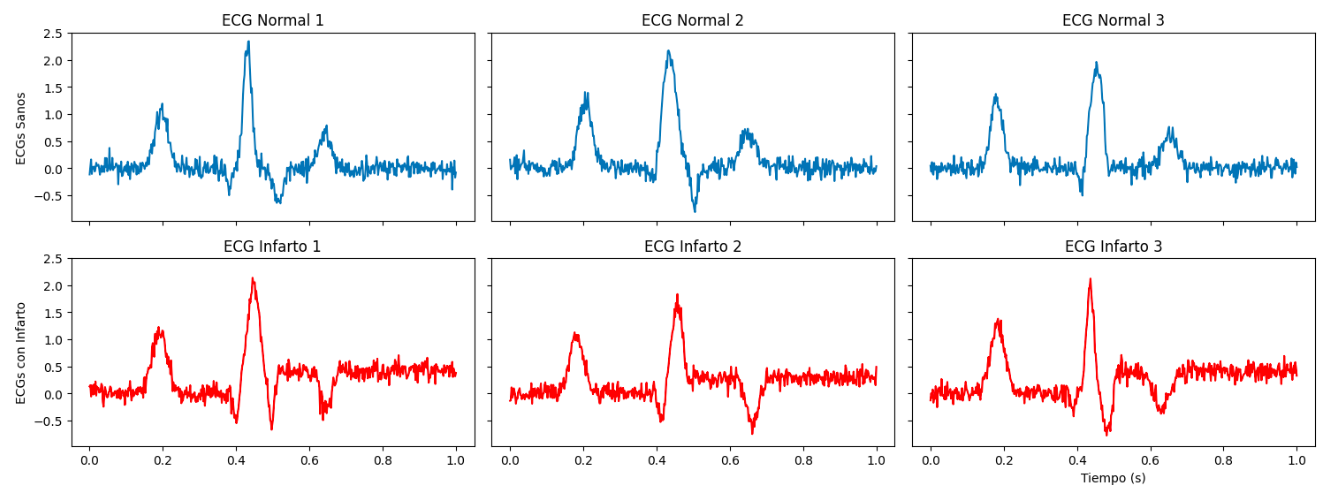
\includegraphics[width=0.9\textwidth]{muestras_sinteticas.png} % Cambia el nombre del archivo
    \caption{Muestras sintéticas de un segundo de señal}
    \label{fig:mi_figura} % Etiqueta para referenciar la figura en el documento
\end{figure}


\subsection{Formulación matemática del problema}
\subsubsection{Clasificación}
Sea un espacio de entrada \( \mathcal{X} \subseteq \mathbb{R}^n \) y un conjunto de etiquetas \( \mathcal{Y} \), donde \( \mathcal{Y} = \{1, 2, \dots, K\} \) en el caso de clasificación multiclase o \( \mathcal{Y} = \{0,1\} \) en el caso binario. Se asume que los datos de entrenamiento están dados por una muestra de tamaño \( m \):

\[
\mathcal{D} = \{(X_i, y_i)\}_{i=1}^{m} \subseteq \mathcal{X} \times \mathcal{Y}
\]

donde cada \( X_i \in \mathcal{X} \) es un vector de características y \( y_i \in \mathcal{Y} \) es su etiqueta correspondiente.

El objetivo del problema de clasificación es encontrar una función \( f: \mathcal{X} \to \mathcal{Y} \) que minimice el riesgo esperado:

\[
R(f) = \mathbb{E}_{(X,Y) \sim P} [\ell(f(X), Y)]
\]

donde \( P(X,Y) \) es la distribución conjunta de los datos y \( \ell: \mathcal{Y} \times \mathcal{Y} \to \mathbb{R}^+ \) es una función de pérdida, típicamente la pérdida 0-1 definida como:

\[
\ell(y, \hat{y}) =
\begin{cases}
    0, & \text{si } y = \hat{y} \\
    1, & \text{si } y \neq \hat{y}
\end{cases}
\]

Dado que la distribución \( P(X,Y) \) es desconocida, se busca minimizar el riesgo empírico:

\[
R_m(f) = \frac{1}{m} \sum_{i=1}^{m} \ell(f(X_i), y_i)
\]

En nuestro caso, nos enfrentamos a dos problemas distintos de clasificación, ambos con el objetivo de determinar si un paciente está sano o no.  

El primero utiliza como entradas los antecedentes clínicos y la información tabular del paciente, mientras que el segundo se basa directamente en las señales de ECG.  

\subsubsection{Reducción de dimensionalidad}
El problema de reducción de dimensionalidad consiste en encontrar una representación de los datos en un espacio de menor dimensión preservando su estructura y contenido informativo. Sea \( X \) un conjunto de datos en un espacio de alta dimensión \( \mathbb{R}^n \), es decir,

\[
X = \{X_i \in \mathbb{R}^n\}_{i=1}^{m},
\]

donde \( m \) es el número de observaciones y \( n \) la cantidad de características. La tarea de reducción de dimensionalidad busca encontrar una transformación

\[
\Phi: \mathbb{R}^n \to \mathbb{R}^d, \quad d \ll n,
\]

de modo que la información relevante contenida en \( X \) se preserve en el espacio reducido \( Z = \Phi(X) \), minimizando la pérdida de información y preservando las relaciones estructurales de los datos.



Un supuesto fundamental en el estudio de la reducción de dimensionalidad es la \textbf{hipótesis de variedades}, la cual postula que los datos de alta dimensión no están distribuidos de manera arbitraria en \( \mathbb{R}^n \), sino que residen en una variedad diferenciable \( \mathcal{M} \) de dimensión \( d \) tal que

\[
\mathcal{M} \subset \mathbb{R}^n, \quad \dim(\mathcal{M}) = d \ll n.
\]

Bajo esta hipótesis, se asume la existencia de una parametrización local \( \psi: \mathbb{R}^d \to \mathbb{R}^n \) que describe la estructura intrínseca de los datos, de modo que cada punto en la variedad puede representarse como

\[
X = \psi(Z), \quad Z \in \mathbb{R}^d.
\]

El objetivo de la reducción de dimensionalidad es encontrar la transformación inversa \( \Phi: \mathbb{R}^n \to \mathbb{R}^d \), la cual extrae una representación compacta de los datos en el espacio latente \( \mathbb{R}^d \).


\section{Metodología}
\subsection{Modelo propuesto}
\subsubsection{Estimación de afinidad a contrar afecciones cardíacas}
Utilizamos un modelo de regresión logística para calcular la probabilidad de que un paciente desarrolle una patología cardíaca en función de características básicas de su estilo de vida. De esta manera, solo almacenamos la estimación de la probabilidad de estar sano o enfermo, la cual servirá como \textit{prior} en los siguientes modelos.

\subsubsection{Aprendizaje de Topología}
Es importante destacar que la distancia euclídea no representa adecuadamente la diferencia entre dos señales temporales, ya que no considera posibles desfasajes. Por esta razón, empleamos la métrica \textit{Dynamic Time Warping} (DTW).

En esta etapa de aprendizaje no supervisado, buscamos encontrar un espacio latente que represente fielmente la estructura de los datos mediante un grafo embebido en el espacio de entrada. Posteriormente, utilizaremos este grafo para aproximar la salida de un nuevo dato. Proponemos dos enfoques distintos para su construcción.

\begin{figure}[H]
    \centering
    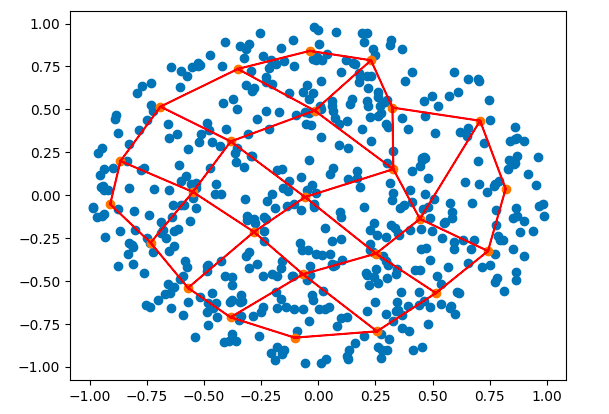
\includegraphics[width=0.8\textwidth]{uniforme_circulo.png}
    \caption{Grafo embebido aprendido mediante SOM}
    \label{fig:mi_figura}
\end{figure}

\subsubsection{SOM}
La arquitectura de la red de Kohonen proporciona de manera natural la estructura de grafo que buscamos.

\subsubsection{K-means}
Otra alternativa consiste en aplicar el algoritmo K-means para encontrar $k$ centroides en los datos, que servirán como nodos del grafo. Luego, dependiendo de los hiperparámetros $\mathbb{d}$ y $\mathbb{\epsilon}$, se pueden conectar los nodos de dos maneras:  
\begin{itemize}
    \item Conectar cada nodo a sus $\mathbb{d}$ vecinos más cercanos.
    \item Conectar cada nodo con todos los que se encuentren a una distancia menor que $\mathbb{\epsilon}$.
\end{itemize}

\subsubsection{Clasificador Probabilístico}
Una vez aprendida esta representación en forma de grafo, para predecir la salida de una nueva entrada, la aproximamos por su centroide más cercano. Para la clasificación, empleamos una \textit{Probabilistic Neural Network} (PNN), donde la distancia se define mediante la distancia geodésica dentro del grafo. Consideramos que esta métrica es más robusta que la distancia euclídea debido a la \textit{maldición de la dimensionalidad}. Así, obtenemos una estimación de la probabilidad de pertenencia a cada clase.

Desde el punto de vista computacional, solo es necesario almacenar una matriz de probabilidades de pertenencia a cada clase según el centroide. Por lo tanto, el costo computacional de realizar una predicción se reduce a encontrar el centroide más cercano, lo cual, aprovechando la estructura de datos \textit{Ball-Tree}, tiene un costo de $\mathcal{O}(\log k)$.

Una ventaja de utilizar un clasificador generativo es que, si la función de pérdida no trata todos los errores de igual forma, como en nuestro caso, podemos tomar la decisión óptima de Bayes, garantizando la minimización de la pérdida.

Desde otra perspectiva, este modelo puede entenderse como una subdivisión del espacio de entrada mediante una teselación de Voronoi basada en los centroides, donde a cada celda se le asigna la probabilidad de que su centroide pertenezca a cada clase.

\begin{figure}[H] % [h] indica que se intenta colocar la imagen aquí
    \centering
    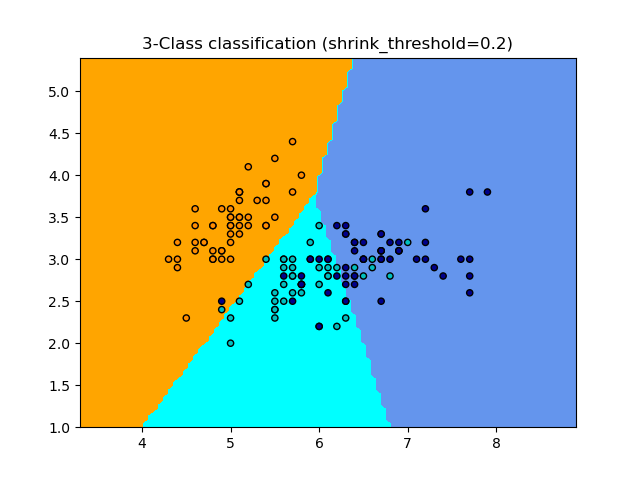
\includegraphics[width=0.6\textwidth]{frontera de decision.png} % Cambia el nombre del archivo
    \caption{ilustrastición de la frontera de decisión ficticia}
    \label{fig:mi_figura} % Etiqueta para referenciar la figura en el documento
\end{figure}

\subsection{Ajuste de hiperparámetros}
Debido a la alta flexibilidad del modelo propuesto, es importante ajustar los hiperparámetros para nuestro problema en cuestión. Usando validación cruzada (Cross-Validation), evaluamos las siguientes combinaciones:

Para la versión con \textbf{K-means}:  
\begin{itemize}
    \item $\sigma \in \{1, 5, 0.2\}$
    \item $n\_neighbors \in \{5, 15, 2\}$
\end{itemize}

Para \textbf{SOM}:  
\begin{itemize}
    \item $\sigma \in \{0.1, 2, 3, 7\}$
    \item learning\_rate $\in \{0.1, 0.5, 1\}$
    \item neighborhood\_function $\in \{\text{gaussian, bubble, mexican\_hat}\}$
\end{itemize}

Como resultado, los valores óptimos fueron:
\begin{itemize}
    \item Para \textbf{K-means}: $\sigma = 5$ y $n\_neighbors = 2$
    \item Para \textbf{SOM}: $\sigma = 7$, learning\_rate $= 0.5$ y neighborhood\_function = mexican\_hat
\end{itemize}

\section{Resultados}
En todos los casos, dividimos los datos en conjuntos de train y test, usando una proporcion de 80-20, respectivamente.

En cuanto al entrenamiento de la regresión logística , la única consideración que tuvimos que tener fue normalizar los datos. Luego, obtuvimos una efectividad del 70 por ciento. 

\subsection{Muestra sintética}
Vemos que ambos modelos muestran una gran efectividad frente a la muestra generada artificialmente. Con tan solo 8 y 16, los modelos de Kmeans y SOM, respectivamente, obtuvieron los siguientes resultados.

\begin{figure}[H] % [h] indica que se intenta colocar la imagen aquí
    \centering
    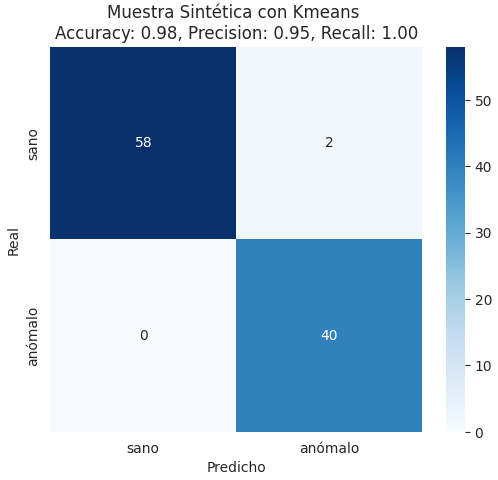
\includegraphics[width=0.5\textwidth]{test_kmeans_sintetico.png} % Cambia el nombre del archivo
    \caption{Predicciones del modelo utilizando Kmeans en la muestra sintética}
    \label{fig:mi_figura} % Etiqueta para referenciar la figura en el documento
\end{figure}
Se puede apreciar como la onda anómala presenta elevación ST y una onda T invertida, característica de un infarto de miocardio.

\begin{figure}[H] % [h] indica que se intenta colocar la imagen aquí
    \centering
    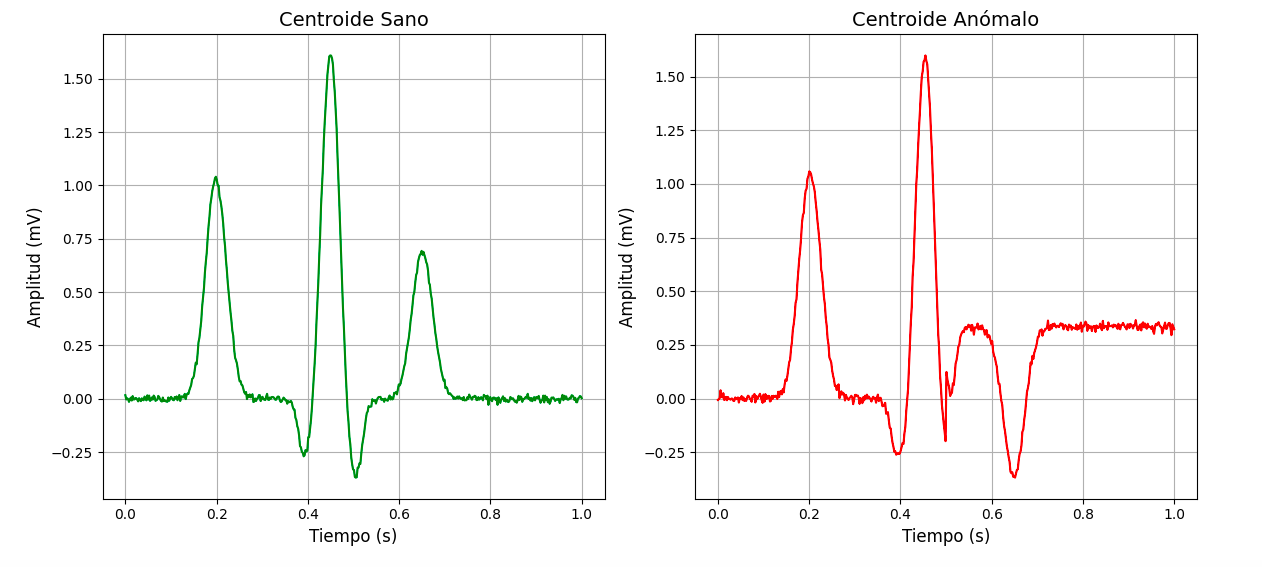
\includegraphics[width=0.8\textwidth]{ecg_centroides_sinteticos.png} % Cambia el nombre del archivo
    \caption{Centroides aprendidos mediante Kmeans de la muestra sintética}
    \label{fig:mi_figura} % Etiqueta para referenciar la figura en el documento
\end{figure}
Utilizando la misma representación que aprendió el modelo podemos visualizar en su espacio latente tanto los datos como los centroides.

\begin{figure}[H] % [h] indica que se intenta colocar la imagen aquí
    \centering
    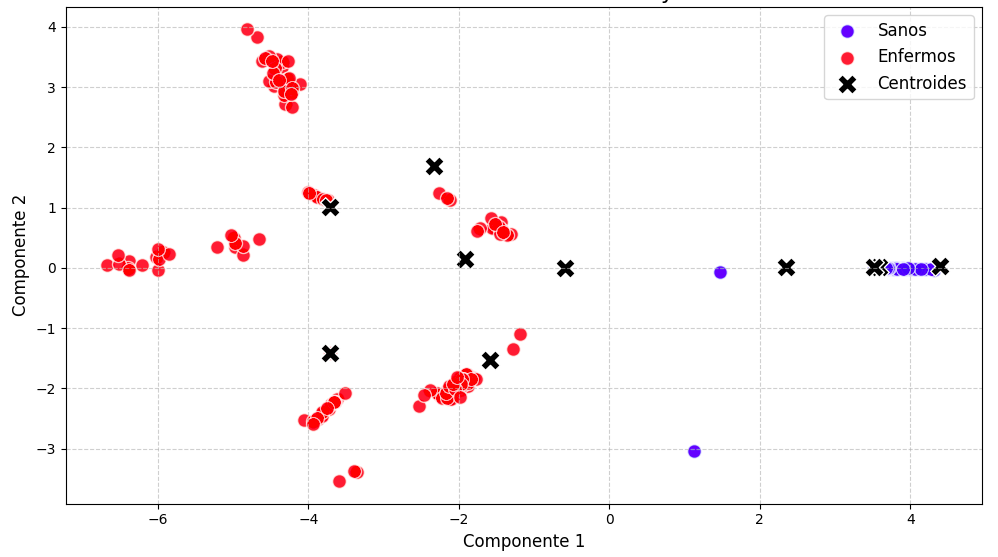
\includegraphics[width=0.8\textwidth]{visualizacion_kmeans_sinteticos.png} % Cambia el nombre del archivo
    \caption{Visualización del espacio latente aprendido con Kmeans de la muestra sintética}
    \label{fig:mi_figura} % Etiqueta para referenciar la figura en el documento
\end{figure}

\subsection{Datos reales}
En general, debido a la naturaleza multimodal de los datos, fue necesario utilizar más centroides en la muestra real para poder obtener una representación efectiva. Entrenamos con 10 centroides en el caso de Kmeans y 25 en el caso de SOM.

\begin{figure}[H] % [h] indica que se intenta colocar la imagen aquí
    \centering
    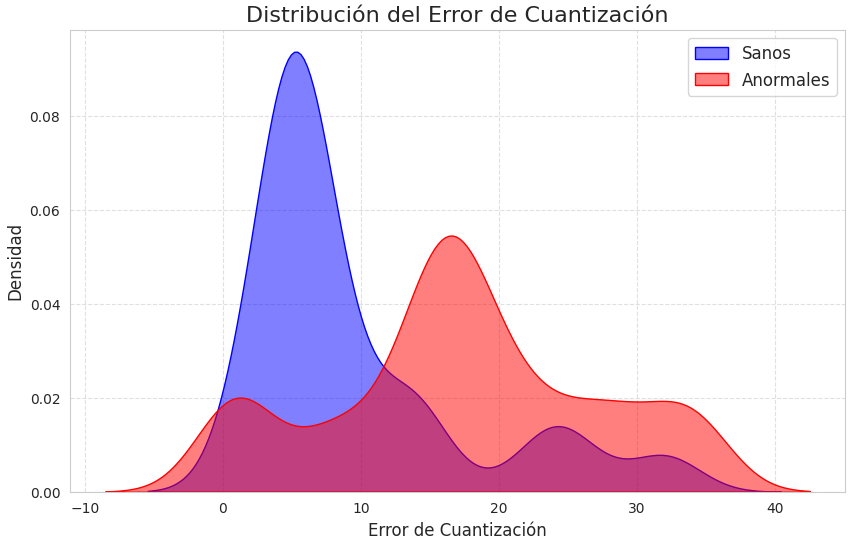
\includegraphics[width=0.7\textwidth]{distribuciones_error.png} % Cambia el nombre del archivo
    \caption{Distribuciones de los errores de aproximación de los datos por su centroide más cercano}
    \label{fig:mi_figura} % Etiqueta para referenciar la figura en el documento
\end{figure}
Cabe destacar, que consistentemente encontramos diferencias en las distribuciones de los errores de aproximación por los datos sanos y anómalos. Esto da evidencia de la diferencia en las distribuciones marginales de cada clase.

\begin{figure}[H] % [h] indica que se intenta colocar la imagen aquí
    \centering
    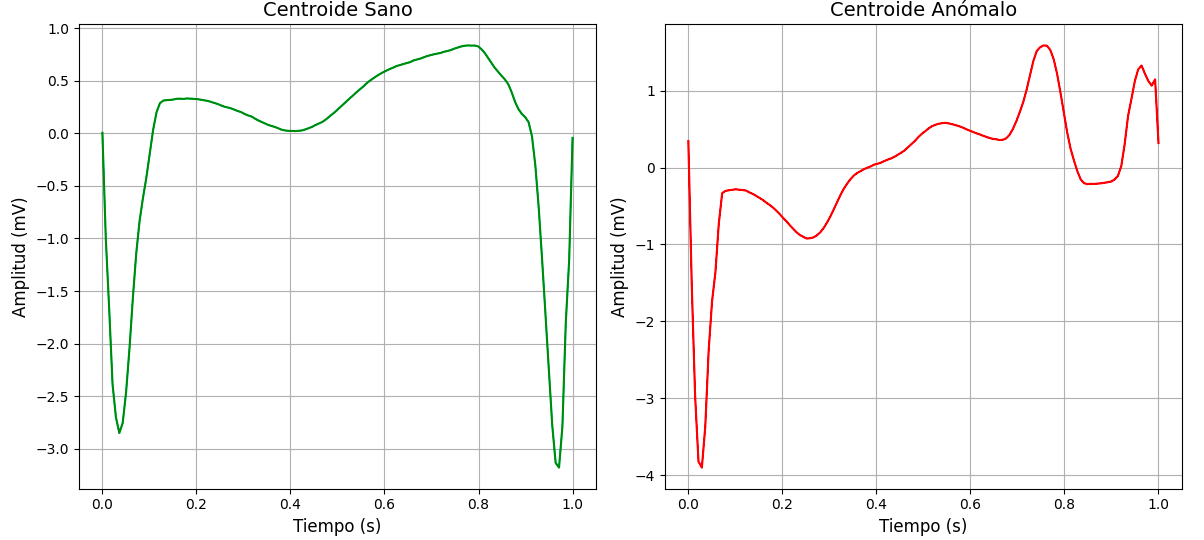
\includegraphics[width=0.7\textwidth]{centroides_kmeans_real.png} % Cambia el nombre del archivo
    \caption{Centroides aprendidos mediante Kmeans de la muestra real}
    \label{fig:mi_figura} % Etiqueta para referenciar la figura en el documento
\end{figure}

\begin{figure}[H] % [h] indica que se intenta colocar la imagen aquí
    \centering
    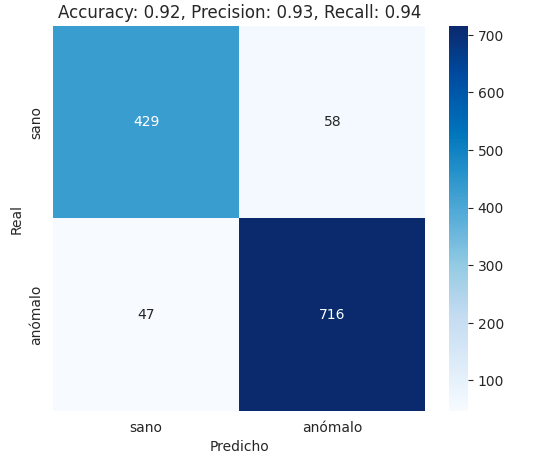
\includegraphics[width=0.7\textwidth]{test_som_real.png} % Cambia el nombre del archivo
    \caption{Matriz de confusión SOM en muestra real}
    \label{fig:mi_figura} % Etiqueta para referenciar la figura en el documento
\end{figure}
\begin{figure}[H] % [h] indica que se intenta colocar la imagen aquí
    \centering
    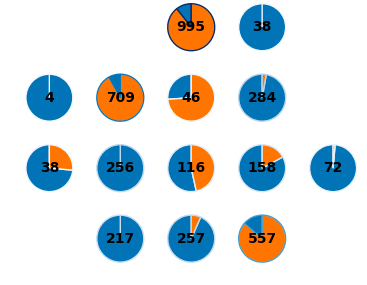
\includegraphics[width=0.5\textwidth]{visualizacion_som.png} % Cambia el nombre del archivo
    \caption{Centroides dispuestos según la reda de kohonen con sus cantidades de datos a los cuales aproximan, en azul proporción de sanos y en naranja proporción de anómalos.}
    \label{fig:mi_figura} % Etiqueta para referenciar la figura en el documento
\end{figure}
Se puede observar una leve mejoría al incorporar la información del estilo de vida de las personas en la efectividad del modelo.
\begin{table}[H]
    \centering
    \begin{tabular}{|c|c|c|c|}
        \hline
        \textbf{Accuracy} & \textbf{Muestra sintética} & \textbf{Muestra real} & \textbf{Muestra real + antecedentes} \\ \hline
        \textbf{SOM} & 0.97 & 0.92 & 0.93 \\ \hline
        \textbf{K-means} & 0.98 & 0.94 & 0.95 \\ \hline
    \end{tabular}
    \caption{Accuracy de los modelos SOM y K-means en diferentes muestras.}
    \label{tab:accuracy}
\end{table}
\begin{table}[H]
    \centering
    \begin{tabular}{|c|c|c|c|}
        \hline
        \textbf{Precisión} & \textbf{Muestra sintética} & \textbf{Muestra real} & \textbf{Muestra real + antecedentes} \\ \hline
        \textbf{SOM} & 0.94 & 0.90 & 0.94 \\ \hline
        \textbf{K-means} & 0.95 & 0.92 & 0.98 \\ \hline
    \end{tabular}
    \caption{Precisión de los modelos SOM y K-means en diferentes muestras.}
    \label{tab:precision}
\end{table}
\begin{table}[H]
    \centering
    \begin{tabular}{|c|c|c|c|}
        \hline
        \textbf{Recall} & \textbf{Muestra sintética} & \textbf{Muestra real} & \textbf{Muestra real + antecedentes} \\ \hline
        \textbf{SOM} & 1.0 & 0.96 & 0.94 \\ \hline
        \textbf{K-means} & 1.0 & 0.98 & 0.92 \\ \hline
    \end{tabular}
    \caption{Recall de los modelos SOM y K-means en diferentes muestras.}
    \label{tab:precision}
\end{table}
\subsection{Discusiones y conclusiones}
En primer lugar, no se está considerando ningún tipo de preprocesamiento de la señal. Implementar esta etapa podría ayudar a reducir el ruido y a preservar los atributos más relevantes de la onda.  

Además del entrenamiento previo basado en electrocardiogramas de distintos individuos, sería posible reajustar el modelo utilizando datos específicos de cada usuario, lo que podría mejorar su precisión en casos particulares.  

Por último, otra posible mejora consistiría en robustecer el modelo entrenándolo con una base de datos que incluya pacientes en movimiento, permitiendo así una mejor generalización ante variaciones dinámicas en las señales.

En conclusión, ambos modelos demostraron un desempeño altamente satisfactorio en términos de precisión y capacidad de clasificación. Su naturaleza generativa permite la incorporación de distintos priors y funciones de pérdida, lo que los hace extremadamente flexibles y adaptables a diferentes escenarios clínicos. Además, presentan una alta eficiencia computacional en la fase de predicción, con un costo de $O(\log(k))$, sin necesidad de emplear más de $k=25$ centroides.

Otro aspecto clave es su elevada interpretabilidad, lo que facilita la comprensión de los patrones aprendidos y su aplicación en un entorno médico. Esto es especialmente relevante para la detección de anomalías cardíacas, donde la transparencia del modelo es fundamental para la confianza y validación por parte de especialistas
\section{Apéndice}
\subsection{Regresión logística}
La regresión logística es un modelo de clasificación que se utiliza cuando la variable de salida \( Y \) es binaria, es decir, \( Y \in \{0,1\} \). En este caso, el objetivo es modelar la probabilidad condicional de pertenencia a una clase dada una entrada \( X \in \mathbb{R}^n \).

La función de probabilidad de la regresión logística está dada por la función sigmoide:

\[
P(Y=1 \mid X) = \frac{1}{1 + e^{-(\beta_0 + \beta^T X)}}
\]

donde:
- \( X \in \mathbb{R}^n \) es el vector de características,
- \( \beta \in \mathbb{R}^n \) es el vector de coeficientes del modelo,
- \( \beta_0 \) es el término de sesgo (bias).

Dado un conjunto de entrenamiento con \( m \) observaciones \( (X_i, y_i) \), la función de verosimilitud del modelo es:

\[
L(\beta) = \prod_{i=1}^{m} P(y_i \mid X_i)^{y_i} (1 - P(y_i \mid X_i))^{1 - y_i}
\]

Tomando el logaritmo de la verosimilitud, obtenemos la función de log-verosimilitud:

\[
\ell(\beta) = \sum_{i=1}^{m} \left[ y_i \log P(y_i \mid X_i) + (1 - y_i) \log (1 - P(y_i \mid X_i)) \right]
\]

Para encontrar los parámetros \( \beta \), se resuelve el problema de optimización:

\[
\hat{\beta} = \arg\max_{\beta} \ell(\beta)
\]

Este problema se resuelve mediante algoritmos numéricos como el descenso de gradiente o el método de Newton-Raphson, ya que no existe una solución cerrada para la optimización de \( \ell(\beta) \).

En el caso de un problema de clasificación con más de dos clases, la regresión logística se generaliza a la **regresión logística multinomial.

\subsection{Dynamic Time Warping}
\textbf{Dynamic Time Warping} (DTW) es un algoritmo utilizado para medir la similitud entre dos secuencias temporales que pueden estar desfasadas en el tiempo. Es ampliamente usado en reconocimiento de patrones, procesamiento de señales y series temporales.

Dadas dos secuencias \( X = (x_1, x_2, \dots, x_n) \) y \( Y = (y_1, y_2, \dots, y_m) \), el DTW busca una alineación no lineal entre ellas minimizando la distancia acumulada en una matriz de costo \( D(i,j) \), definida recursivamente como:

\[
D(i,j) = d(x_i, y_j) + \min 
\begin{cases}
    D(i-1, j) \\
    D(i, j-1) \\
    D(i-1, j-1)
\end{cases}
\]

donde \( d(x_i, y_j) \) es una función de distancia, comúnmente la distancia euclidiana. Utilizando programacion dinamica se logra tener una complejidad lineal en el tamano de la entrada.

\subsection{Kmeans}
El algoritmo \( k \)-means es un método de agrupamiento no supervisado que busca particionar un conjunto de datos en \( k \) grupos minimizando la variabilidad intra-clúster.



Dado un conjunto de datos \( X = \{x_1, x_2, \dots, x_m\} \subset \mathbb{R}^n \), el objetivo es encontrar una partición \( C = \{C_1, \dots, C_k\} \) y centroides \( \{\mu_1, \dots, \mu_k\} \) tales que se minimice la función de costo:

\[
J = \sum_{j=1}^{k} \sum_{x_i \in C_j} \|x_i - \mu_j\|^2.
\]

\begin{algorithm}
\caption{K-Means Clustering}
\begin{algorithmic}[1]
\State \textbf{Input:} Dataset $\{x_1, x_2, \dots, x_n\}$, number of clusters $k$, and maximum number of iterations $T$
\State \textbf{Output:} Cluster centers $\{\mu_1, \mu_2, \dots, \mu_k\}$
\State Initialize the $k$ cluster centers randomly: $\mu_1, \mu_2, \dots, \mu_k$
\For{$t = 1 \text{ to } T$}
    \For{each point $x_i$ in the dataset}
        \State Assign $x_i$ to the cluster $C_j$ where:
        \[
        C_j = \arg \min_{1 \leq j \leq k} \left\| x_i - \mu_j \right\|^2
        \]
    \EndFor
    \For{each cluster $C_j$}
        \State Update the center $\mu_j$ as:
        \[
        \mu_j = \frac{1}{|C_j|} \sum_{x_i \in C_j} x_i
        \]
    \EndFor
\EndFor
\State \textbf{Return} the final cluster centers $\mu_1, \mu_2, \dots, \mu_k$
\end{algorithmic}
\end{algorithm}

El algoritmo \( k \)-means es eficiente (\( O(m k n) \) por iteración), pero depende de la inicialización de los centroides y puede quedar atrapado en mínimos locales. Métodos como \( k \)-means++ mejoran la selección inicial de centroides.

\subsection{SOM}
Los \textbf{Self-Organizing Maps} (SOM) son redes neuronales no supervisadas que se utilizan para la reducción de dimensionalidad y la visualización de datos de alta dimensión. Organizan los datos en una cuadrícula de nodos y actualizan los pesos de los nodos según la proximidad a los datos de entrada.

\begin{algorithm}
\caption{Algoritmo de Self-Organizing Maps (SOM)}
\begin{algorithmic}[1]
\State \textbf{Inicialización:}
\State \quad Inicializar los pesos de los nodos aleatoriamente.
\State \quad Establecer la tasa de aprendizaje inicial $\eta_0$ y el radio de vecindad inicial $r_0$.

\For{cada iteración $t$}
    \For{cada dato de entrada $\mathbf{x}$}
        \State Calcular la distancia entre $\mathbf{x}$ y los pesos de los nodos: $d_i = || \mathbf{x} - \mathbf{w}_i(t) ||$ para todos los nodos $i$.
        \State Identificar el nodo ganador $\mathbf{w}_\text{BMU}(t)$, donde $d_\text{BMU} = \min \{ d_1, d_2, \dots, d_n \}$.
        \State Para cada nodo $i$, actualizar los pesos:
        \[
        \mathbf{w}_i(t+1) = \mathbf{w}_i(t) + \eta(t) \cdot h_{i, \text{BMU}}(t) \cdot (\mathbf{x} - \mathbf{w}_i(t))
        \]
        donde $h_{i, \text{BMU}}(t)$ es la función de vecindad que depende de la distancia entre el nodo $i$ y el BMU.

    \EndFor
    \State Reducir la tasa de aprendizaje $\eta(t)$ y el radio de vecindad $r(t)$.
\EndFor
\end{algorithmic}
\end{algorithm}

\begin{itemize}
    \item \( N \): Número de puntos de datos.
    \item \( M \): Número de nodos en la cuadrícula del mapa.
    \item \( D \): Dimensionalidad de los datos de entrada.
    \item \( T \): Número de iteraciones o ciclos de entrenamiento.
\end{itemize}

La complejidad comutacional del algoritmo es 
\[
O(T \cdot N \cdot M \cdot D)
\]
\subsection{Probabilistic Neural Network}
\textbf{Probabilistic Neural Networks} (PNN) son un tipo de red neuronal basada en la teoría de estimación de densidad de probabilidad, utilizada principalmente en problemas de clasificación. Se derivan del clasificador de máxima verosimilitud y emplean funciones de base radial (RBF) para estimar la probabilidad de cada clase.

Un PNN consta de cuatro capas principales:

\begin{itemize}
    \item \textbf{Capa de entrada}: Recibe el vector de características de la muestra de entrada.
    \item \textbf{Capa de patrones}: Contiene un nodo por cada muestra de entrenamiento y aplica una función kernel, típicamente la gaussiana:
    \[
    f_i(\mathbf{x}) = \frac{1}{(2\pi)^{d/2} \sigma^d} \exp\left(-\frac{||\mathbf{x} - \mathbf{x}_i||^2}{2\sigma^2}\right)
    \]
    \item \textbf{Capa de suma}: Agrupa los valores de la capa de patrones según la clase a la que pertenecen.
    \item \textbf{Capa de decisión}: Asigna la clase con la mayor probabilidad estimada según la regla de Bayes.
\end{itemize}


La decisión se basa en la minimización de la \textbf{esperanza de la función de pérdida} \( L(C_k, \hat{C}) \), definida como:

\[
\hat{C} = \arg\min_k \mathbb{E}[L(C_k, \hat{C}) | \mathbf{x}]
\]

\subsection{Ball-Tree}
\textbf{Ball-Tree} es una estructura jerárquica utilizada para búsqueda eficiente de vecinos más cercanos (\textit{k-nearest neighbors}, KNN) en espacios métricos. A diferencia de los \textit{k-d trees}, que dividen el espacio con hiperplanos, los Ball-Trees utilizan hiperesferas para particionar los datos.


Cada nodo del Ball-Tree contiene:
\begin{itemize}
    \item Un \textbf{centro} \( c \), que es el centroide de los puntos en el nodo.
    \item Un \textbf{radio} \( r \), que es la distancia máxima desde \( c \) a cualquier punto del nodo.
    \item Dos nodos hijos en los que se divide el conjunto de puntos.
\end{itemize}


\begin{algorithm}
\caption{Construir\_Ball\_Tree(\( P \))}
\begin{algorithmic}[1]
\Require Conjunto de puntos \( P \)
\Ensure Nodo raíz del Ball-Tree

\If{\( |P| \leq \) UMBRAL} 
    \State Crear un nodo hoja con los puntos en \( P \).
    \State \Return Nodo hoja.
\EndIf
\State Calcular el centroide \( c \) de \( P \).
\State Calcular el radio \( r \) como la distancia máxima de \( c \) a los puntos en \( P \).
\State Elegir dos puntos lejanos y dividir \( P \) en \( P_L \) y \( P_R \).
\State Crear un nodo con centro \( c \) y radio \( r \).
\State Asignar recursivamente los nodos hijos:
\State \( \text{nodo.izquierdo} \gets \text{Construir\_Ball\_Tree}(P_L) \)
\State \( \text{nodo.derecho} \gets \text{Construir\_Ball\_Tree}(P_R) \)
\State \Return Nodo creado.
\end{algorithmic}
\end{algorithm}


\begin{algorithm}
\caption{Buscar\_Vecinos(\( \text{nodo}, q, S \))}
\begin{algorithmic}[1]
\Require Nodo actual, punto de consulta \( q \), lista de mejores candidatos \( S \)
\Ensure Lista \( S \) con los \( k \) vecinos más cercanos

\If{nodo es hoja} 
    \For{cada punto \( p \) en el nodo} 
        \State Calcular la distancia \( d(q, p) \).
        \State Si \( d(q, p) \) es menor que la peor distancia en \( S \), actualizar \( S \).
    \EndFor
    \State \Return
\EndIf
\State Determinar el nodo hijo más cercano a \( q \).
\State Llamar recursivamente a Buscar\_Vecinos en el nodo hijo más cercano.
\State Si el nodo hijo lejano puede contener mejores resultados, explorarlo recursivamente.
\State \Return Lista \( S \) actualizada.
\end{algorithmic}
\end{algorithm}


\begin{itemize}
    \item \textbf{Construcción}: \( O(n \log n) \), donde \( n \) es el número de puntos.
    \item \textbf{Búsqueda}: En promedio, \( O(\log n) \) en dimensiones bajas, pero puede degradarse a \( O(n) \) en dimensiones altas.
\end{itemize}
\subsection{Teselacion de Voronoi}
Dada una colección de puntos $S = \{ p_1, p_2, \dots, p_k \}$ en $\mathbb{R}^n$, la \textbf{Teselación de Voronoi} divide el espacio en regiones, donde cada región $V_i$ está definida como:
\[
V_i = \{ x \in \mathbb{R}^n \mid d(x, p_i) \leq d(x, p_j), \forall j \neq i \}
\]
donde $d(x, y)$ es la distancia euclidiana entre los puntos $x$ e $y$.

\begin{itemize}
    \item Cada celda de Voronoi es un conjunto convexo.
    \item En $\mathbb{R}^2$, los bordes de las celdas son segmentos de mediatrices.
    \item La intersección de tres o más celdas se llama \textit{vértice de Voronoi}.
    \item La \textbf{dual} de la teselación de Voronoi es el \textbf{diagrama de Delaunay}.
\end{itemize}

\subsection{Cross-Validation}
La \textbf{validación cruzada} es una técnica utilizada en aprendizaje automático para evaluar el rendimiento de un modelo y prevenir el sobreajuste (\textit{overfitting}). Su objetivo es estimar la capacidad de generalización del modelo al probarlo en datos no vistos durante el entrenamiento.


La validación cruzada divide el conjunto de datos en \textit{k} subconjuntos o \textit{folds}. El modelo se entrena \textit{k} veces, usando \textit{k-1} partes para el entrenamiento y la restante para la validación. Al final, se promedian los resultados para obtener una estimación robusta del desempeño.


El método más común es el \textbf{\textit{k}-fold cross validation}, que sigue los siguientes pasos:

\begin{algorithm}
\caption{k-Fold Cross Validation}
\begin{algorithmic}[1]
\Require Conjunto de datos \( D \) y número de pliegues \( k \)
\Ensure Desempeño promedio del modelo

\State Dividir \( D \) en \( k \) subconjuntos de igual tamaño
\State \( \text{rendimientos} \gets [] \)
\For{cada \( i \) de 1 a \( k \)}
    \State \( D_{\text{train}} \gets D \setminus D_i \) \Comment{Entrenar en \( k-1 \) subconjuntos}
    \State \( D_{\text{test}} \gets D_i \) \Comment{Validar en el subconjunto restante}
    \State Entrenar el modelo con \( D_{\text{train}} \)
    \State \( \text{resultado} \gets \text{Evaluar el modelo con } D_{\text{test}} \)
    \State Añadir \( \text{resultado} \) a \( \text{rendimientos} \)
\EndFor
\State \( \text{desempeño\_promedio} \gets \frac{1}{k} \sum_{i=1}^{k} \text{rendimientos}[i] \)
\State \Return \( \text{desempeño\_promedio} \)
\end{algorithmic}
\end{algorithm}
\end{document}
